\lhead{\emph{Motivación}}
\chapter{Motivación}

\section{Introducción}

Los límites físicos de los que adolecen los computadores en la época actual hacen de la computación distribuida y paralela un método para incrementar de forma sencilla y rentable el rendimiento total de un sistema, rendimiento que aumenta significativamente en problemas \textit{ridículamente paralelos}\citationneeded.

Sin embargo, dichos beneficios conllevan una serie de inconvenientes, o el aumento de la complejidad de diversas tareas. En general, un sistema distribuido requiere de un conjunto de máquinas independientes, que en conjunto constituyen un coste superior al de un único nodo. Además, aparecen nuevos problemas de índole técnica: problemas de comunicación, depuración de aplicaciones, etcétera. Con el objetivo de solventar estos inconvenientes se han propuesto varias soluciones.

\section{Situación actual}

\subsection{Computadores de placa única}

Los computadores de placa única (\textit{Single-Board Computer}) consisten en computadores de generalmente bajas prestaciones que aglutinan todos los componentes necesarios para su funcionamiento en un único circuito integrado. Dichas placas suelen tener un coste bajo y una relación rendimiento/coste muy elevada.

Durante los últimos años se han popularizado como una herramienta para el estudio y creación de sistemas distribuidos con un gran rango de propósitos diferentes.

\subsubsection{RPiCluster (Joshua Kiepert)}

Joshua Kiepert, estudiante de doctorado en la universidad Boise State, crea este sistema utilizando 33 computadores \textbf{Raspberry Pi B}, con el objetivo de utilizarlo como herramienta de pruebas que sirva de alternativa al supercomputador situado en su universidad\cite{joshuarpicluster}, sobre el que trabaja de forma rutinaria, a fin de poder continuar su trabajo en periodos de mantenimiento, cierre del centro, etcétera. El sistema está diseñado para utilizar la \textit{Message Passing Interface} y además poder utilizar los diferentes puertos de las placas (GPIO, I\textsuperscript{2}C, SPI, UART), puertos generalmente ausentes en computadores como clústeres. Utiliza además un servidor \textbf{NFS} para compartir datos entre todos los nodos, y un \textit{router} dedicado para la interconexión. El sistema se complementa con un ordenador \textbf{Chromeboox} con el mismo sistema operativo (\textbf{Arch Linux}), que actúa como nodo coordinador.

%TODO: Diagram here
% http://www.zdnet.com/article/build-your-own-supercomputer-out-of-raspberry-pi-boards/

\begin{figure}[H]
\centering
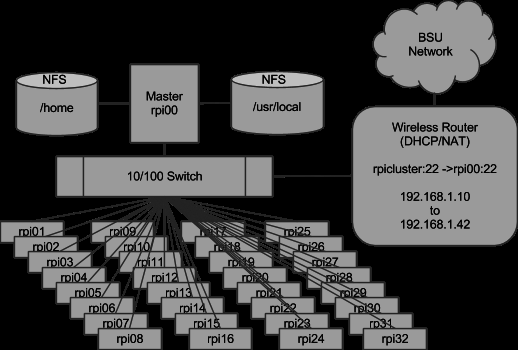
\includegraphics[width=0.5\textwidth]{Chapter1/Figures/structure.png}
\caption{Estructura del sistema (Fuente: Joshua Kiepert).}
\label{kiepert:structure}
\end{figure}

\textbf{Coste}: 1967.21 dólares.


\subsubsection{Dramble (Jeff Geerling)}

El clúster \textit{Dramble} es un conjunto de 6 equipos \textbf{Raspberry Pi} capaces de ejecutar en conjunto el gestor de contenidos \textbf{Drupal}\footnote{\href{https://www.drupal.org/}{drupal.org}}. El sistema es utilizado como servidor de pruebas para la ejecución de instancias de \textbf{Drupal} de forma experimental o durante demonstraciones en público\cite{geerlingraspberry}.

\begin{figure}[H]
\centering
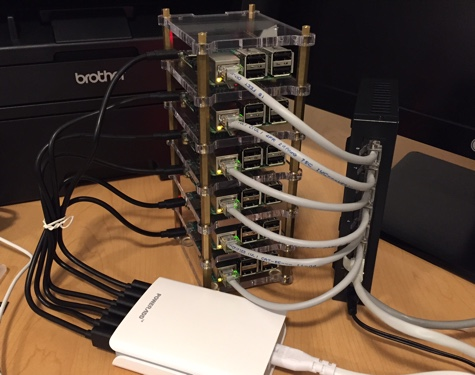
\includegraphics[width=0.5\textwidth]{Chapters/Chapter1/Figures/raspberry-pi-dramble-cluster-wired.jpg}
\caption{El \textit{Dramble} en ejecución}
\label{geerling:dramble}
\end{figure}


\textbf{Coste (estimado)}: 35 dólares por cada Raspberry Pi\citationneeded

\subsubsection{Bramble (GCHQ)}

El organismo gubernamental \textit{Government Communication Headquarters}, agencia de inteligencia del Gobierno Británico presentó en la \textit{Big Bang Fair} de 2015 un proyecto educativo que combina 66 \textit{Raspberry Pi} en un clúster jerárquico con 8 grupos de 8 nodos, cada uno de ellos con un coordinador, y dos nodos coordinadores. El cableado se reduce gracias al uso de la tecnología \textbf{PoE} (\textit{Power over Ethernet}), y cada \textbf{Raspberr} cuenta con un conjunto de elementos adicionales, como un reloj de tiempo real, disco duro externo, cámara, punto de acceso WiFi, etcétera\cite{gchqbramble}.

\begin{figure}[H]
\centering
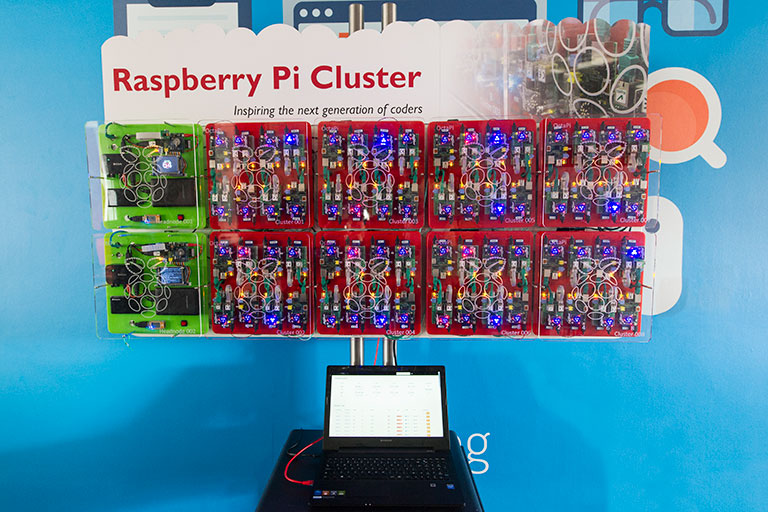
\includegraphics[width=0.5\textwidth]{Chapters/Chapter1/Figures/bramblegchq}
\caption{Vistazo general de la estructura del sistema}
\label{gchq:bramble}

\textbf{Coste (estimado)}\citationneeded

\end{figure}

\subsubsection{Clúster Iridis (Simon Cox, University of Southampton)}

Con el objetivo de atraer a jóvenes estudiantes al mundo de la Computación, el profesor Simon Cox crea este clúster con 64 \textbf{Raspberry Pi B} sobre una estructura de LEGO\cite{cox:raspberry}
%TODO: http://www.i-programmer.info/news/91-hardware/8385-gchq-builds-a-raspberry-pi-cluster.html
\begin{figure}[H]
\centering
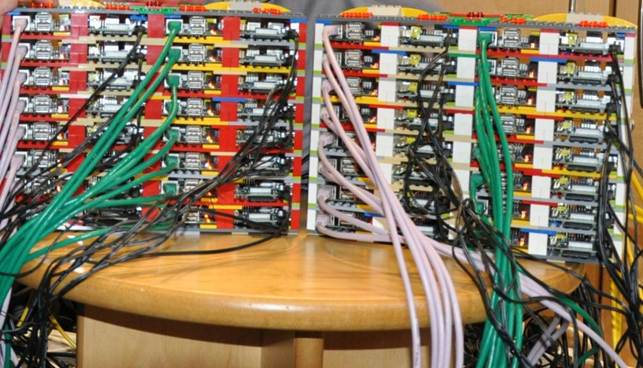
\includegraphics[width=0.5\textwidth]{Chapters/Chapter1/Figures/iridis-pi.jpg}
\caption{Sistema}
\label{cox:iridis}

%w
\end{figure}

\subsubsection{Paralella}

%http://www.zdnet.com/article/parallella-the-99-linux-supercomputer/

%http://www.webstreet.com/super_computer.htm